\documentclass[12pt]{report}
\usepackage[utf8]{inputenc}
\usepackage[spanish]{babel}
\usepackage[spanish=nohyphenation]{hyphsubst}

\usepackage{parskip} 
\usepackage{selinput}
\usepackage{tikz}
\usepackage{blindtext}
\usepackage{csquotes}
\usepackage{graphicx}
\usepackage[font=footnotesize,labelfont=bf,justification=centering,textfont=it]{caption}
\usepackage{float}
\usepackage{hyperref}
\usepackage{tabularx}
\usepackage{longtable}
\usepackage{listings}
\usepackage{color}
\usepackage{amsmath}
\usepackage{mathtools}
\usepackage{datetime}
\usepackage{listingsutf8}
\usepackage{dirtytalk}
\usepackage{mwe}
\usepackage{biblatex}

\addbibresource{references.bib}
% \bibliography{teg/references.bib}
\makeatletter

\lstdefinelanguage{JavaScript}{
  keywords={typeof, new, true, false, catch, function, return, null, catch, switch, var, if, in, while, do, else, case, break},
  keywordstyle=\color{blue}\bfseries,
  ndkeywords={class, export, boolean, throw, implements, import, this},
  ndkeywordstyle=\color{darkgray}\bfseries,
  identifierstyle=\color{black},
  sensitive=false,
  comment=[l]{//},
  morecomment=[s]{/*}{*/},
  commentstyle=\color{purple}\ttfamily,
  stringstyle=\color{red}\ttfamily,
  morestring=[b]',
  morestring=[b]"
}

\lstset {
    language=JavaScript,           % language code
    basicstyle=\footnotesize,      % font size
    numbers=none,                  % where to put line numbers
    numberstyle=\footnotesize,     % numbers size
    numbersep=5pt,                 % how far the line numbers are from the code
    backgroundcolor=\color{white}, % background color
    showspaces=false,              % show spaces (with underscores)
    showstringspaces=false,        % underline spaces within strings
    showtabs=false,                % show tabs using underscores
    frame=single,                  % adds a frame around the code
    tabsize=4,                     % default tabsize
    breaklines=true,               % automatic line breaking
    columns=fullflexible,
    breakautoindent=false,
    framerule=1pt,
    xleftmargin=0pt,
    xrightmargin=0pt,
    breakindent=0pt,
    resetmargins=true
}

\setlength{\parindent}{15pt}
\setlength\bibitemsep{0.5\baselineskip}

\definecolor{lightgray}{rgb}{.9,.9,.9}
\definecolor{darkgray}{rgb}{.4,.4,.4}
\definecolor{purple}{rgb}{0.65, 0.12, 0.82}

\newdateformat{mydate}{\shortmonthname[\THEMONTH], \THEYEAR}

\renewcommand*{\thefootnote}{\arabic{footnote}}

\graphicspath{ {images/} }
\title{
	{Desarrollo de un editor de visualizaciones de propiedades de historiales de wikis}\\
	{\large Universidad Central de Venezuela}\\
}
\author{Adrian J. Mejias O. y Jose E. Tirado S.}



\addto\captionsspanish{
  \renewcommand{\listfigurename}
    {índice de figuras}
  \renewcommand{\listtablename}
    {índice de tablas}
  \renewcommand\lstlistingname{Código Fuente}
  \renewcommand\lstlistlistingname{índice de código fuente}
}
\renewcommand\spanishtablename{Tabla}
\newcommand{\tabitem}{~~\llap{\textbullet}~~}

\begin{document}

\begin{titlepage}
	\centering
	{\large República Bolivariana de Venezuela \par}
	{\large Universidad Central de Venezuela\par}
	{\large Facultad de Ciencias\par}
	{\large Escuela de Computación\par}\vspace{2cm}

	
\includegraphics[scale=0.60]{ucv_logo.png}\par\vspace{1cm}
	{\scshape\Large\textbf{\@title}\par}
	\vfill

    {\large Tutor Prof. Eugenio Scalise \par}
    {\large Pasante subpagado \@author \par}
	{\large \mydate\today \par}
\end{titlepage}

\tableofcontents

\listoffigures

\chapter{Introducción}
% LATE_TODO: Introducción

% introducción: hablar un poco sobre wiki y la filosofía de wiki, también sobre la visualización de datos y terminamos con hablar sobre el trabajo en si

Un wiki es un sitio web que permite a sus usuarios colaborar en su estructura y contenido. Esta versatilidad que provee el concepto de Wiki es lo que lo convierte en una de las herramientas mas usadas en la actualidad para compartir información. La enciclopedia Wikipedia es el sitio web más popular basado en wiki. 

El principal problema que maneja Wikipedia en cuanto a moderación de contenido viene como resultado de su propia filosofía "todos pueden editar", lo que conlleva a multiples problemas tales como: vandalismo, escritura pobre, una mala estructura de página, peleas de edición, entre otras cosas. Por esta razón no existe una solución única para acabar con la existencia de \say{mal} contenido en Wikipedia, y es indispensable el uso de participación humana en procesos de moderación que implican complejos desafíos técnicos y éticos.

En la actualidad, gracias a la evolución del internet, la información es considerada virtualmente ubicua y en constante cambio, y lo que realmente ofrece valor es la capacidad individual de sintetizar esa información y relacionarla. Como resultado de esto surge la filosofía wiki, en donde la información se comparte, y el conocimiento no se crea, sino se co-crea de forma colaborativa.

El concepto de la filosofía de wiki y el software utilizado para crear estos sitios web están intrínsecamente relacionados, y no se podría poner en práctica lo primero sin lo segundo. Esto es así debido a que el software debe proporcionar el medio para que pueda existir esa construcción colectiva de conocimiento, que es indispensable en la filosofía wiki.





\chapter{Marco Teórico}




\section{Visualizacion de datos}

La visualización de datos es la práctica de traducir información en un contexto visual, como un mapa o gráfico, para facilitar que el cerebro humano comprenda y extraiga información útil.\\

Las formas más generales de visualización de datos son las siguientes: Gráficas, Tablas, Mapas, Infografias y Tableros. En este trabajo se hará uso especificamente de gráficas como medio de visualización de datos, ya que los datos obtenidos de Wikipedia no permiten ser visualizados de otra forma.


\subsection{Tipos de gráficas}

\section{Dominio del problema}
    \subsection{Wiki}

        El término wiki proviene de la raiz hawaiana wiki, que significa "rápido", y fue propuesto por Ward Cunningham, quien a su vez define los sitios web wiki como "La base de datos más simple que puede existir" [Cunningham, Ward (June 27, 2002), What is a Wiki]. Con el tiempo el concepto de Wiki fue evolucionando, y hoy en dia cuando hablamos de wiki nos referimos a un sitio web que permite a sus usuarios colaborar en su estructura y contenido.\\
        
        Wikimedia es el nombre colectivo del movimiento wikimedia, que incluye un grupo de proyectos interrelacionados, tales como: Wikipedia, Wiktionary, Wikiquote, Wikibooks, Wikisource, entre otros, cuyo proposito es usar el poder colaborativo de internet, y el concepto wiki, para compartir conocimiento gratuito de cualquier tipo.\\
        
        MediaWiki es el motor que impulsa los sitios web basados en wiki. En este documento se hará efasis en este sistema, debido a que se trabajará con articulos de Wikipedia, quien hace uso de Mediawiki para cumplir con muchas de sus funcionalidades.

    \subsection{Filosofía de la wiki}

        [https://www.um.es/ead/red/M11/intro.pdf]
        [https://ignasialcalde.es/filosofia-wiki-y-dinamicas-relacionales/]
        
        Antes de la existencia del internet, la información era poder, y saber mucho era tener mucha información. En esos tiempos la información era en su mayoria fisica y centralizada, lo que le otorgaba muchisimo valor. En la actualidad la información es considerada virtualmente ubicua y en constante cambio, y lo que realmente ofrece valor es la capacidad individual de sintetizar esa información y relacionarla, además de saber utilizar esa información con un fin.

        Basandose en el principio anteriormente mencionado es que surge la filosofía de wiki, en donde la información de comparte, y el conocimiento no se crea, sino se co-crea de forma colaborativa.

    \subsection{Watcher}

    \subsection{Wikipedia como ejemplo práctico}

    \subsection{Visualizacion cientifica}


\subsection{Tecnologias a utilizar}

    Para la realización de este proyecto se usaran las siguientes tecnologias:

    \subsubsection{ReactJS}

        ReactJS es una librería de JavaScript de código abierto desarrollada por Facebook para facilitar la creación de componentes interactivos, reutilizables, para desarrollos de interfaces de usuario, especialmente aplicaciones de una sola página.

        React maneja el concepto de \say{programación reactiva} haciendo uso de un DOM Virtual, lo le permite determinar qué partes del DOM han cambiado comparando contenidos entre la versión nueva y la almacenada den el DOM virtual, para así propagar los datos generando cambios en la aplicación, es decir, los datos \say {reaccionan} ejecutando una serie de eventos.\\

        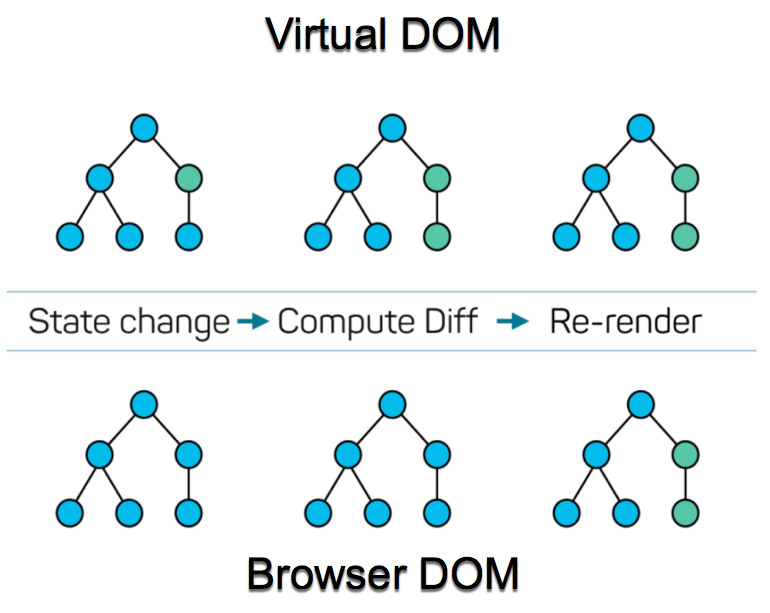
\includegraphics[scale=0.5]{virtual_dom}\\

        Este concepto de reactividad es lo que hace a la libreria altamente eficiente, ya que limita la actualización del DOM solamente a los elementos que han cambiado.
        
    \subsubsection{SEO}
    
        Se trata del proceso de mejorar un sitio web en relación con los motores de búsqueda. También representa el cargo de la persona que trabaja en este proceso: Acabamos de contratar a un nuevo SEO para que mejore nuestra presencia en la Web.

    \subsubsection{NextJS}
        NextJS es un framework desarrollado encima de Node.js que permite a las aplicaciones de React usar funcionalidades como el renderizado del lado de servidor o la generación estática de paginas, que permite realizar aplicaciones con mejor desempeño en cuanto a SEO.


    \subsubsection{Fastify}

    \subsubsection{Mongo}

        MongoDB es un sistema de base de datos NoSQL, orientado a documentos y de código abierto. En lugar de guardar los datos en tablas, tal y como se hace en las bases de datos relacionales, MongoDB guarda estructuras de datos BSON (una especificación similar a JSON) con un esquema dinámico, haciendo que la integración de los datos en ciertas aplicaciones sea más fácil y rápida.

        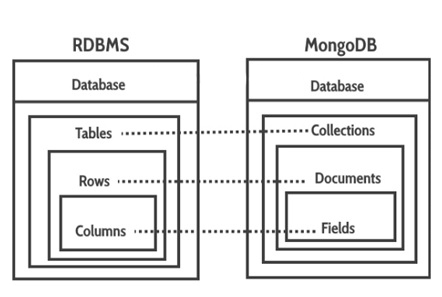
\includegraphics{mongodb-structure.jpg}


\subsection{Metodologias agiles}


    \subsubsection{Frameworks}

    \begin{enumerate}
        \item Kanban: Tiene como objetivo la mejora continua, la flexibilidad en la gestión de tareas y un flujo de trabajo mejorado. Con este enfoque ilustrativo, el progreso de todo el proyecto se puede comprender fácilmente de un vistazo. Para esto hace uso del tablero Kanban, que es una herramienta que visualiza todo el proyecto para rastrear el flujo de su proyecto. A través de este enfoque gráfico de los tableros Kanban, un miembro nuevo o una entidad externa puede comprender lo que está sucediendo en este momento, las tareas completadas y las tareas futuras.
        \item Scrum: Es un framework para desarrollo, entrega, y mantenimiento de proyectos en un ambiente complejo, con un enfasis inicial en el desarrollo de software, aunque tambien ha sido utilizado en otras areas como la investigación, ventas, mercadeo y tecnologías avanzadas. Esta diseñado para equipos de 10 personas o menos, quienes rompen su trabajo en metas que pueden ser completadas en iteraciones de tiempo fijo, llamadas \emph{sprints}, con duraciones aproximadas de 2 semanas. 
        \item Extreme programming (XP)
        \item Lean software development: Es un framework popular basado en optimizar tiempo de desarrollo y recursos, eliminando desperdicios y entregando solamente lo que el producto necesita. El método Lean es usualmente referido como la estrategia del \say{Producto Minimo Viable (PMV)}, 
        estrategia, en la que un equipo lanza una versión mínima de su producto al mercado, aprende de los usuarios lo que les gusta, lo que no les gusta y lo que quieren que se agregue, y luego itera en función de estos comentarios.
        \item Adaptive Software Development (ASD):
        \item Rapid application development (RAD)
    \end{enumerate}

    \subsubsection{Prácticas}

    \begin{enumerate}
        \item Backlogs (Product and Sprint)
        \item Continuous integration (CI)
        \item Daily Stand-up / Daily Scrum
        \item Domain-driven design (DDD)
        \item Acceptance test-driven development (ATDD)
        \item Iterative and incremental development (IID)
        \item Planning poker
        \item Refactoring
        \item Pair programming
        \item Specification by example
        \item Agile modeling
        \item Agile testing
        \item Behavior-driven development (BDD)
        \item Cross-functional team
        \item Scrum events (sprint planning, sprint review and retrospective)
        \item Story-driven modeling
        \item Test-driven development (TDD)
        \item Timeboxing
        \item User story
        \item Velocity tracking
    \end{enumerate}



\chapter{Marco Teórico}
Para el análisis de datos, el paso fundamental es la visualización de estos, dado que sin una imagen clara de la información a trabajar, los especialistas no pueden comparar grupos de datos de forma eficiente. 

"La visualización de datos es la práctica de traducir información en un contexto visual, como un mapa o gráfico, para facilitar que el cerebro humano comprenda y extraiga información útil". \cite{DefinitionDataViz}

De esta manera se facilita la identificación, localización de errores, patrones y cualquier punto a resaltar para su próxima conclusión.

Esta tarea además de importante es compleja por lo cual necesita de agrupaciones que se encarguen de trabajar en ella constantemente. Estas agrupaciones publican sus esfuerzos en plataformas como Github para así poder aportar a la investigación, discutir soluciones, revisar problemas y atraer nuevos colaboradores que permitan el crecimiento y consiguiente eficacia del trabajo.

En esta sección se busca investigar y comparar esos productos probados, refinados y simplificados para dar con la que mejor se adapte para los requerimientos a cubrir. 

\section{Librerías o frameworks para aplicaciones intensivas de frontend}

%LATE_TODO

\section{Librerías para la visualización de datos}
Pero no cualquier librería 
Para la selección de librería se consideran los siguientes factores:

\begin{enumerate}
    \item {Debe ser un proyecto open source.}
    \item {De ser posible, debe tener bindings para ReactJS para facilidad en el desarrollo.}
    \item {Debe ser extensible para poder implementar aquellas visualizaciones que sean muy específicas.}
    \item {Deben ser longevas y tener cierta garantía de que será mantenida en el tiempo,
    asegurando así que para futuras mejoras de este TEG sigan disponibles.}
    \item {Debe ser fácil de utilizar}
\end{enumerate}

\subsection{ Data Driven Documents (D3) }
\begin{itemize}
    \item URL de repositorio \href{https://github.com/d3/d3}{https://github.com/d3/d3}
    \item Mantenida por la organización homónima, d3
\end{itemize}

\subsection{ echarts }
\begin{itemize}
    \item URL de repositorio \href{https://github.com/apache/echarts}{https://github.com/apache/echarts}
    \item Mantenida por Apache
\end{itemize}

\subsection{ Comparación de bibliotecas }

Después de comparar estas librerías, sus APIs y leer otras investigaciones la decisión final es utilizar echarts

La base de esta conclusión es la simplicidad \cite{EchartsDecision}, mientras que d3 permite una gran flexibilidad, la curva de aprendizaje tiene una inclinación pronunciada. 
En comparación, echarts se ve como una herramienta plug and play que requiere mínima configuración y ahorra al desarrollador días de esfuerzo.

El tipo de gráficas a utilizar son las siguientes
\begin{itemize}    
    \item Número
    \item Línea
    \item Barra
    \item Área
    \item Torta
    \item Dispersión
    \item History flow
\end{itemize}

Para estas gráficas echarts provee soluciones pre-hechas y si es el caso de gráficos de interés en nichos específicos, como es el caso del History Flow, permite que fácilmente crees gráficas completamente nuevas. 
También provee gráficos de Sankey y Stacked Area Chart que son bastante parecidos y podrían ser personalizados para parecerse al History Flow. 

\section{ Proyectos alternos }
Estos dos gigantes en el mundo de la visualización de datos por si solos son opciones excelentes, pero trabajan sobre JavaScript vainilla y no están adaptadas para trabajar directamente sobre tecnologías como ReactJS. 
Para facilidad del desarrollo de la aplicación se utilizará una librería que se encargue de adaptar echarts a ReactJS.

\subsection{ echarts for react }
\begin{itemize}
    \item URL del repositorio \href{https://github.com/hustcc/echarts-for-react}{https://github.com/hustcc/echarts-for-react}
\end{itemize}

\chapter{Marco Tecnológico}
\section{Dominio del problema}

    Para la realización de este proyecto se usarán las siguientes tecnologías:

    \subsection{ReactJS}

        ReactJS es una librería de JavaScript de código abierto desarrollada por Facebook para facilitar la creación de componentes interactivos, reutilizables, para desarrollos de interfaces de usuario, especialmente aplicaciones de una sola página.\\

        React maneja el concepto de \say{programación reactiva} haciendo uso de un DOM Virtual, lo le permite determinar qué partes del DOM han cambiado comparando contenidos entre la versión nueva y la almacenada den el DOM virtual, para así propagar los datos generando cambios en la aplicación, es decir, los datos \say {reaccionan} ejecutando una serie de eventos.\\

        Este concepto de reactividad es lo que hace a la librería altamente eficiente, ya que limita la actualización del DOM solamente a los elementos que han cambiado.\\

        Otras características que destacan en React son:\\

        \begin{itemize}
            \item \textbf{Componentes} \hfill \\

            El código de React es hecho con entidades llamadas componentes. Los componentes pueden ser renderizados en elementos particulares del DOM usando la libreria de React DOM. Estos componentes son capaces de recibir parametros conocidos como "propiedades del componente" de la siguiente forma: \hfill \\

            \begin{lstlisting}
                ReactDOM.render(<Greeter greeting="Hello World!" />, document.getElementById('myReactApp'));
            \end{lstlisting}

            Las 2 formas de declarar componentes en react es mediante el uso de funciones o clases, y generalmente se usa una de las dos opciones de forma situacional.

            \item \textbf{JSX} \hfill \\

            JSX, tambien llamado Javascript XML, es una extension a la sintaxis del lenguaje javascript. Este provee una forma de estructurar componentes usando una sintexis familiar para muchos desarrolladores. Los componentes de React son usualmente escritos usando JSX, aunque tambien pueden ser escritos usando Javascript puro.

            Un ejemplo de codigo JSX:

            \begin{lstlisting}
                class App extends React.Component {
                    render() {
                        return (
                        <div>
                            <p>Header</p>
                            <p>Content</p>
                            <p>Footer</p>
                        </div>
                        );
                    }
                }
            \end{lstlisting}

            \item \textbf{Hooks} \hfill \\

            Los hooks son funciones que permiten a los desarrolladores \say{engancharse} a los estados de React y a ciertos puntos dentro del ciclo de vida de los componentes.

            React proporciona algunos hooks integrados tales como: useState, useContext, useReducer, useMemo y useEffect, los cuales son los mas usados y permiten controlar los estados y eventos respectivamente.


        \end{itemize}
        
    \subsection{Next.js}

        Next.js es un framework desarrollado encima de Node.js que permite a las aplicaciones de React usar funcionalidades como el renderizado del lado servidor y la generación de paginas web estáticas.\\

        Por defecto, Next.js pre-renderiza cada pagina. Esto significa que Next.js genera HTML para cada pagina en adelanto, en vez de hacerse con Javascript del lado del cliente. Pre-renderizado puede resultar en mejor rendimiento y SEO.\\

        Cada HTML generado es asociado con el mínimo código Javascript necesario para que funcione la pagina. Cuando una página es cargada en el explorador, su código javascript se ejecuta y hace la página totalmente interactiva. A este proceso de le conoce como \say{hydration}

        Next.js ofrece 2 formas de pre-renderizado: 

        \begin{itemize}
            \item Generación estática: El HTML es generado a tiempo de ejecución y será reutilizado en cada petición.
            \item Renderizado lado servidor: El HTML es generado en cada petición
        \end{itemize}

    \subsection{MongoDB}

        MongoDB es un sistema de base de datos NoSQL, orientado a documentos y de código abierto. En lugar de guardar los datos en tablas, tal y como se hace en las bases de datos relacionales, MongoDB guarda estructuras de datos BSON (una especificación similar a JSON) con un esquema dinámico, haciendo que la integración de los datos en ciertas aplicaciones sea más fácil y rápida.

        \iffalse 
            \begin{figure}
                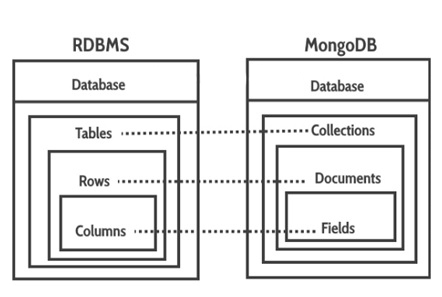
\includegraphics[scale=1.2]{mongodb-structure.jpg}
                \caption{Comparación de estructura de datos entre MongoDB y los RDBMS (sistema de gestión de bases de datos relacionales)}
            \end{figure}
        \fi

    \subsection{Fastify}

        Fastify es un framework web para Node.js de código abierto concentrado en proporcionar el mejor rendimiento, y una arquitectura flexible. \\

        Si comparamos la velocidad de fastify con otros frameworks web como express, tal como podemos ver en la figura \ref{fig:fastify_vs_express}, notamos que fastify es aproximadamente un 20\% más rápido que express. \\

        \begin{figure}
            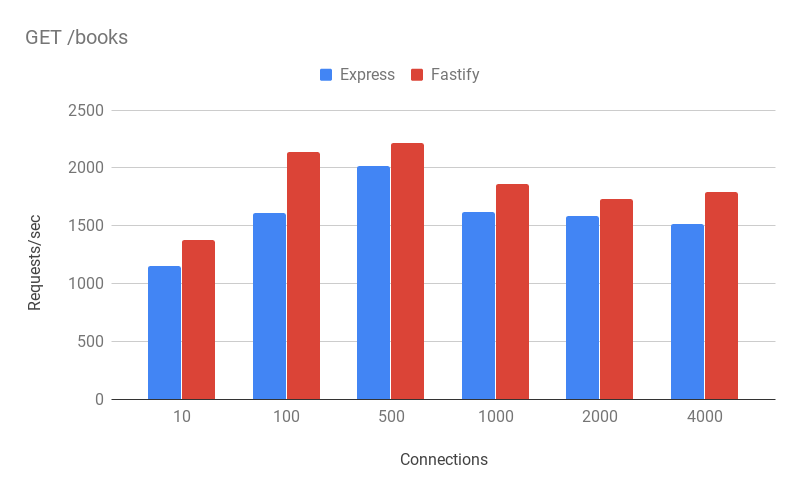
\includegraphics[scale=0.5]{fastify_vs_express.png}
            \caption{ Número de peticiones por segundo para distinta cantidad de conexiones}
            \label{fig:fastify_vs_express}
        \end{figure}
    


\section{Metodologias ágiles}

    \section{Frameworks}

    \begin{enumerate}
        \item Kanban: Tiene como objetivo la mejora continua, la flexibilidad en la gestión de tareas y un flujo de trabajo mejorado. Con este enfoque ilustrativo, el progreso de todo el proyecto se puede comprender fácilmente de un vistazo. Para esto hace uso del tablero Kanban, que es una herramienta que visualiza todo el proyecto para rastrear el flujo de su proyecto. A través de este enfoque gráfico de los tableros Kanban, un miembro nuevo o una entidad externa puede comprender lo que está sucediendo en este momento, las tareas completadas y las tareas futuras.
        \item Scrum: Es un framework para desarrollo, entrega, y mantenimiento de proyectos en un ambiente complejo, con un enfasis inicial en el desarrollo de software, aunque tambien ha sido utilizado en otras areas como la investigación, ventas, mercadeo y tecnologías avanzadas. Esta diseñado para equipos de 10 personas o menos, quienes rompen su trabajo en metas que pueden ser completadas en iteraciones de tiempo fijo, llamadas \emph{sprints}, con duraciones aproximadas de 2 semanas. 
        \item Lean software development: Es un framework popular basado en optimizar tiempo de desarrollo y recursos, eliminando desperdicios y entregando solamente lo que el producto necesita. El método Lean es usualmente referido como la estrategia del \say{Producto Minimo Viable (PMV)}, 
        estrategia, en la que un equipo lanza una versión mínima de su producto al mercado, aprende de los usuarios lo que les gusta, lo que no les gusta y lo que quieren que se agregue, y luego itera en función de estos comentarios.
        \item Extreme programming (XP): Es una metodología de desarrollo de software cuyo objetivo es mejorar la calidad del software y la adaptabilidad al cambio de los requerimientos del cliente. Al ser un tipo de metodología agil, se basa en el uso de ciclos de desarrollo cortos con lanzamientos frecuentes, con el proposito de de mejorar la productividad e introducir \say{checkpoints} en los que se puedan adoptar nuevos requisitos de clientes.
        \item Adaptive Software Development (ASD): Es una consecuencia directa del desarrollo agil. Su objetivo es permitir que los equipos se adapten rápida y eficazmente a los requisitos cambiantes o las necesidades del mercado mediante la evolución de sus productos con una planificación ligera y un aprendizaje continuo. El enfoque ASD alienta a los equipos a desarrollarse de acuerdo con un proceso de tres fases: especular, colaborar, aprender. 
        \item Rapid application development (RAD):  es una forma de metodología de desarrollo de software ágil que prioriza las versiones e iteraciones rápidas de prototipos. A diferencia del método Waterfall, RAD enfatiza el uso de software y los comentarios de los usuarios sobre la planificación estricta y el registro de requisitos.
    \end{enumerate}


\chapter{Propuesta de Trabajo Especial de Grado}


\section{Motivación e identificación del problema}

El orgullo de Wikipedia como la mayor fuente información (en forma de artículos sobre eventos, personajes, definiciones, conceptos, locaciones y entre otros...) se debe a su extensa red de colaboradores.

Cada vez que estos ejecutan una acción en la wikipedia -ya sea si aportan artículo complejo o corrigen una tilde- dejan una huella llamada metadata. Estos "rastros", conformados por fechas, numero de lineas editadas, direcciones IP y demás, son de suma importancia para analistas de datos; 


% TODO: Porque este trabajo es un trabajo util
% Aprovechar la data que genera wikipedia
% wikipedia tiene apis
% sacarle provecho
% apoyar a los watchers en su labor de vigilancia de sus artículos


\section{Objetivos del trabajo}


\subsection{Objetivo General}
% TODO : Hacer Objetivo General
Crear una nueva version del front-end de wikimetrics y extender con funcionalidades pertinentes para fomentar discusión sobre los artículos

\subsection{Objetivos Específicos}
% TODO: Objectivos Específicos

\begin{itemize}
    \item Implementar una aplicación web responsive que ofrezca las funcionalidades requeridas por un watcher de un wiki y que pueda ser reconocida por los motores de búsqueda.
    \item Consumir y extender la API de wikimetrics para desarrollar una aplicación web que habilite a sus usuarios construir y visualizar gráficas
    \item Definir los requerimientos de la aplicación
    \item Utilizar un método ágil para el desarrollo de la aplicación.
    \item Realizar el despliegue y puesta en producción de la aplicación
\end{itemize}

\section{Estrategia de solución y método de desarrollo ágil a utilizar}

\subsection{Desarrollo Rápido de Aplicaciones (RAD)}

El desarrollo rápido de aplicaciones es una metodología de desarrollo que prioriza la creación rápida y prototipos y la retroalimentación rápida sobre ciclos prolongados de desarrollo y prueba. Con el uso de RAD, los desarrolladores pueden realizar multiples iteraciones y actualizaciones al software rápidamente sin la necesidad de iniciar un cronograma de desarrollo desde cero cada vez.

Esta metodología de desarrollo fue creada por James Martin en el año 1980 en IBM y fue formalizada con la publicación del libro \emph{Rapid Application Development} en 1991.

\begin{figure}[H]
    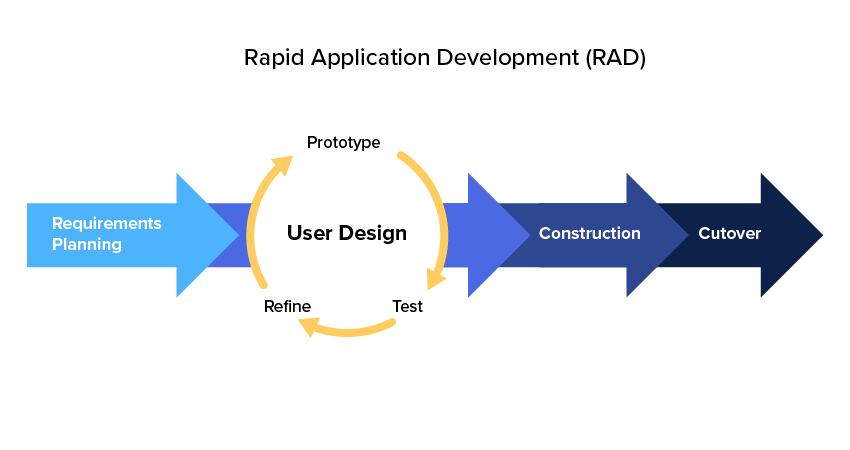
\includegraphics[scale=0.45]{Rapid-application-development.png}
    \caption{Fases del Desarrollo Rápido de Aplicaciones (enfoque de James Martin)}
    \label{fig:Rapid-application-development}
\end{figure}

\subsubsection{Fases del Desarrolo Rápido de Aplicaciones}

Según el enfoque de James Martin \cite{RADJamesMartin} el Desarrollo Rápido de Aplicaciones se divide en las siguientes fases:

\begin{itemize}
    \item \textbf{Fase de planificación:} Esta fase es equivalente a una reunión de alcance del proyecto. Aunque la fase de planificación se condensa en comparación con otras metodologías de gestión de proyectos.

          Durante esta etapa, los desarrolladores, los clientes (usuarios de software) y los miembros del equipo se comunican para determinar los objetivos y las expectativas del proyecto, así como los problemas actuales y potenciales que deben abordarse durante la construcción.

    \item \textbf{Fase de diseño:} Durante esta fase, los usuarios interactúan con analistas de sistemas y desarrollan modelos y prototipos que representan todos los procesos, entradas y salidas del sistema.

          Todos los errores y problemas se resuelven en un proceso iterativo. El desarrollador diseña un prototipo, el cliente (usuario) lo prueba y luego se reúnen para comunicar qué funcionó y qué no.

    \item \textbf{Fase de construcción:} Esta etapa toma los prototipos y el sistema en su fase beta resultado de la etapa de diseño y lo convierte en un modelo funcional.

          Debido a que la mayoría de los problemas y cambios se abordaron durante la minuciosa fase de diseño iterativo, los desarrolladores pueden construir el modelo de trabajo final más rápidamente que siguiendo un enfoque tradicional de gestión de proyectos.

    \item \textbf{Fase de transición:} Esta es la fase de implementación donde el producto terminado va al lanzamiento. Incluye conversión de datos, pruebas y cambio al nuevo sistema, así como capacitación de usuarios.

          Todos los cambios finales se realizan mientras los programadores y los clientes continúan buscando errores en el sistema.

\end{itemize}


\section{Trabajos similares, diferencias y ventajas de la solución a desarrollar}

Siendo Wikimedia y Wikipedia las mas grandes comunidades y organizaciones dedicadas a recopilar datos, es lógico pensar que tiene consigo una abundante cantidad de seguidores capacitados y apasionados por aportar lo que puedan. A continuación se detallará el estado actual de las herramientas existentes para explorar la Wikipedia.

Estas herramientas cumplen diferentes objetivos,

\begin{enumerate}
    \item Identificar posibles candidatos para ser administrador
    \item Identifica
    \item Etc.
\end{enumerate}


\subsection{Toolforge}

\begin{itemize}
    \item URL del proyecto \url{https://wikitech.wikimedia.org/wiki/Portal:Toolforge}
\end{itemize}

Comenzando con el proyecto madre de Wikimedia, este gigante sirve de plataforma para que colaboradores técnicos puedan usar servidores de Wikipedia para desarrollo y para poder levantar aplicaciones que mejoren la experiencia de todos los colaboradores de Wikipedia.
\\
Este proyecto es particularmente interesante porque podría ser un medio por el cual la aplicación WikiMetaView y sus dependencias podrían ser servidas al público.

\url{https://www.wikidata.org/wiki/Wikidata:Tools/Visualize_data}

\subsection{Sigma - ArticleInfo}
\begin{itemize}
    \item URL del proyecto \url{https://sigma.toolforge.org/articleinfo.py}
\end{itemize}

\begin{figure}[H]
    \centering
    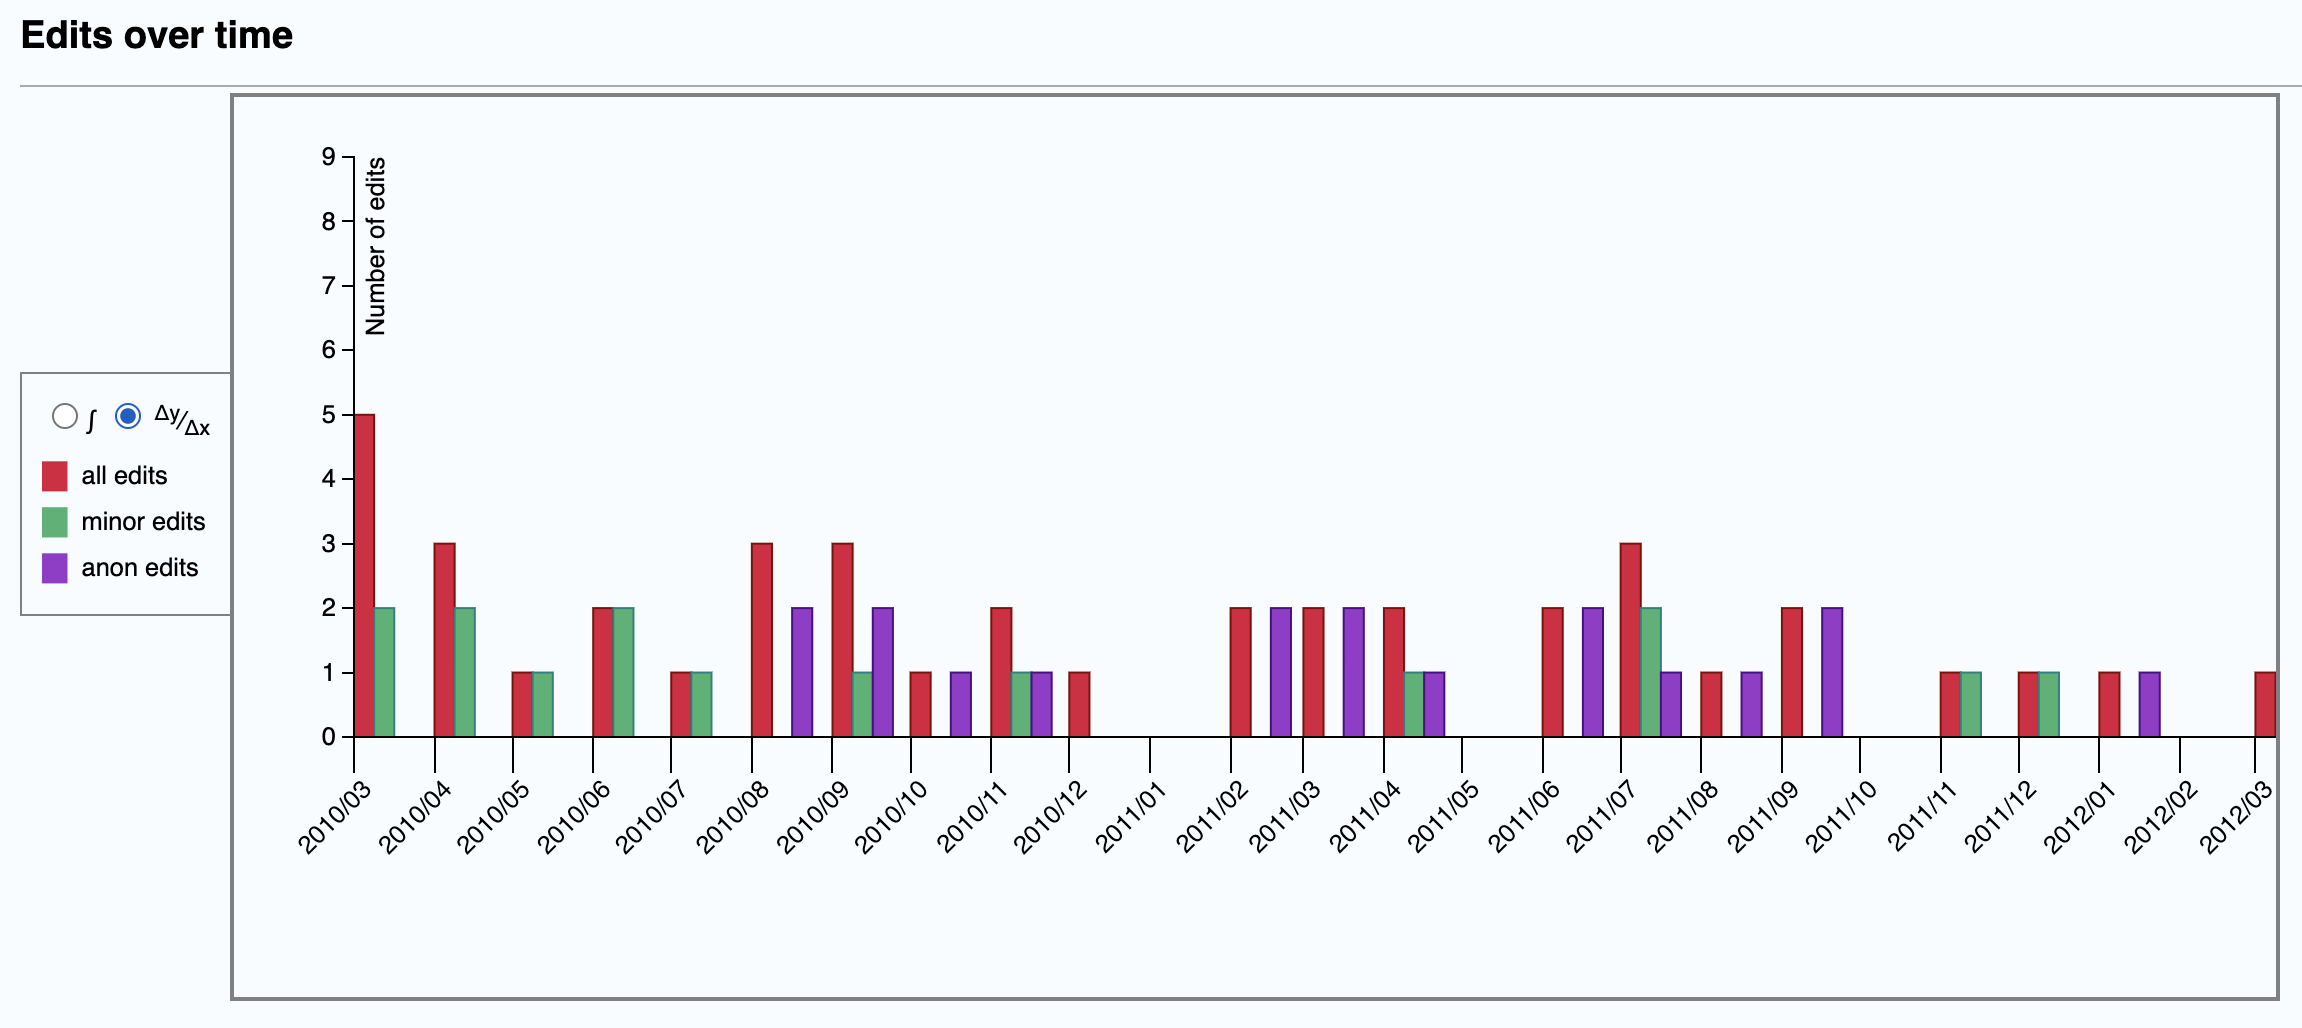
\includegraphics[width=1.0\textwidth]{proyectos relacionados/sigma_article-info.png}
    \caption{Sigma Article Info}
    \label{sigma_articleInfo}
\end{figure}


% This isn't really useful lol
% \url{https://interaction-timeline.toolforge.org/}

\subsection{Histropedia Timeline}

\begin{itemize}
    \item URL del proyecto \url{http://histropedia.com/timeline/}
\end{itemize}

Es una herramienta que permite visualizar diferentes eventos en forma de linea de tiempo interactiva, usando el servicio de Wikidata para consultas Sparql \cite{WikidataSparql}. Es usada como herramienta educativa por distintas entidades como el Museo del Prado para que los usuarios puedan visualizar de forma sencilla el arte que se expone, tal como se puede observar en la imagen \ref{fig:museo-de-prado-timeline}. Ademas la linea te tiempo permite asociar cada elemento de la colleción con un evento historico importante, de tal forma que se facilite el aprendizaje y se haga más dinámico.

\begin{figure}[H]
    \centering
    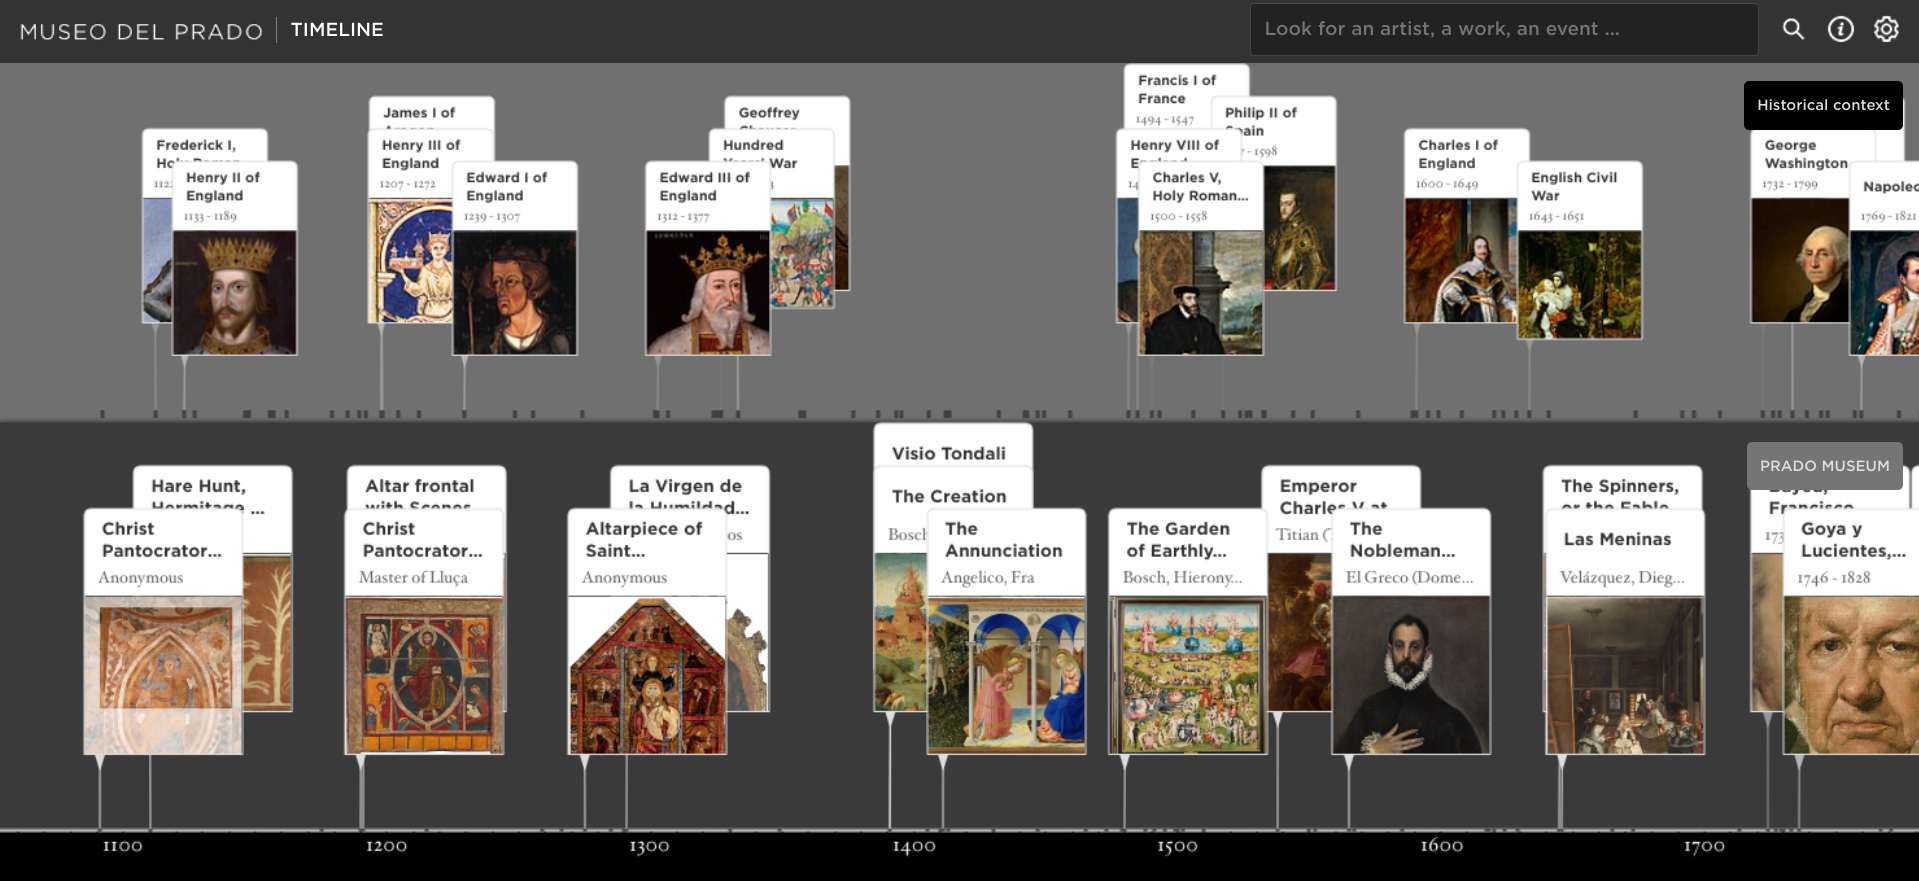
\includegraphics[width=1.0\textwidth]{proyectos relacionados/museo-del-prado-timeline.png}
    \caption{Linea de tiempo que muestra la colección de arte del Museo del Prado}
    \label{fig:museo-de-prado-timeline}
\end{figure}



\begin{figure}[H]
    \centering
    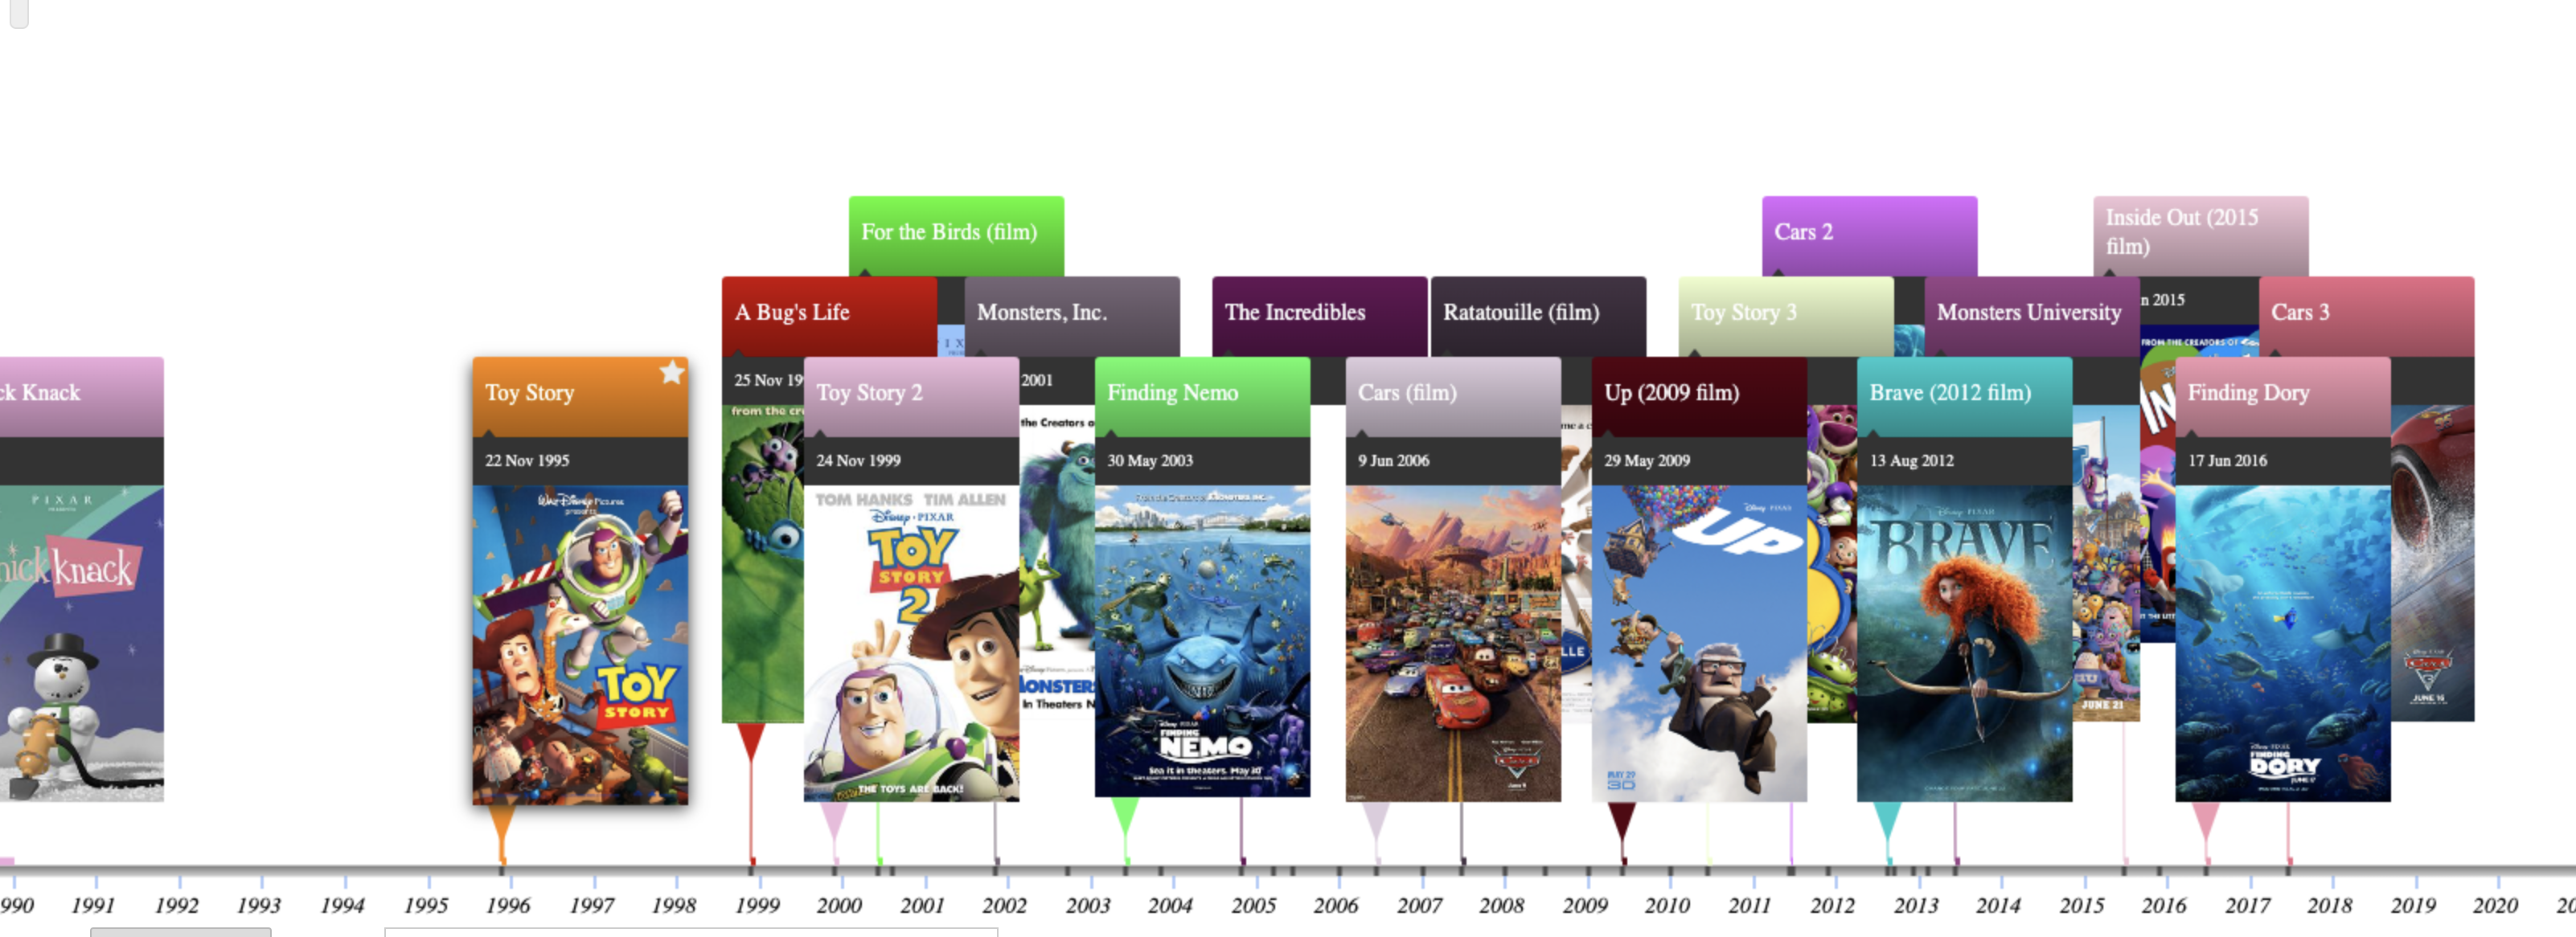
\includegraphics[width=1.0\textwidth]{proyectos relacionados/histropedia_timeline.png}
    \caption{Histropedia Timeline}
    \label{histropedia_timeline}
\end{figure}


\url{https://en.wikipedia.org/wiki/Wikipedia:Tools}

\url{apersonbot.toolforge.org}
Este set de herramientas esta enfocado en supervisar usuarios y sus contribuciones a la Wikipedia

- Candidate Search
- Aadminscore
- Articles for Creation Review History

\subsection{Xtools}
\begin{itemize}
    \item URL del proyecto \url{https://xtools.wmflabs.org/}
\end{itemize}

\subsection{Wiki Replay}
\begin{itemize}
    \item URL del proyecto \url{https://cosmiclattes.github.io/wikireplay/player}
\end{itemize}

Se encarga de mostrar una linea de tiempo con los cambios en un articulo. Esta linea de tiempo
tiene el comportamiento de un reproductor de video y permite que el usuario presione un botón de
reproducir y así ser guiado por como el contenido de un artículo ha ido evolucionando en el tiempo.

\begin{figure}[H]
    \centering
    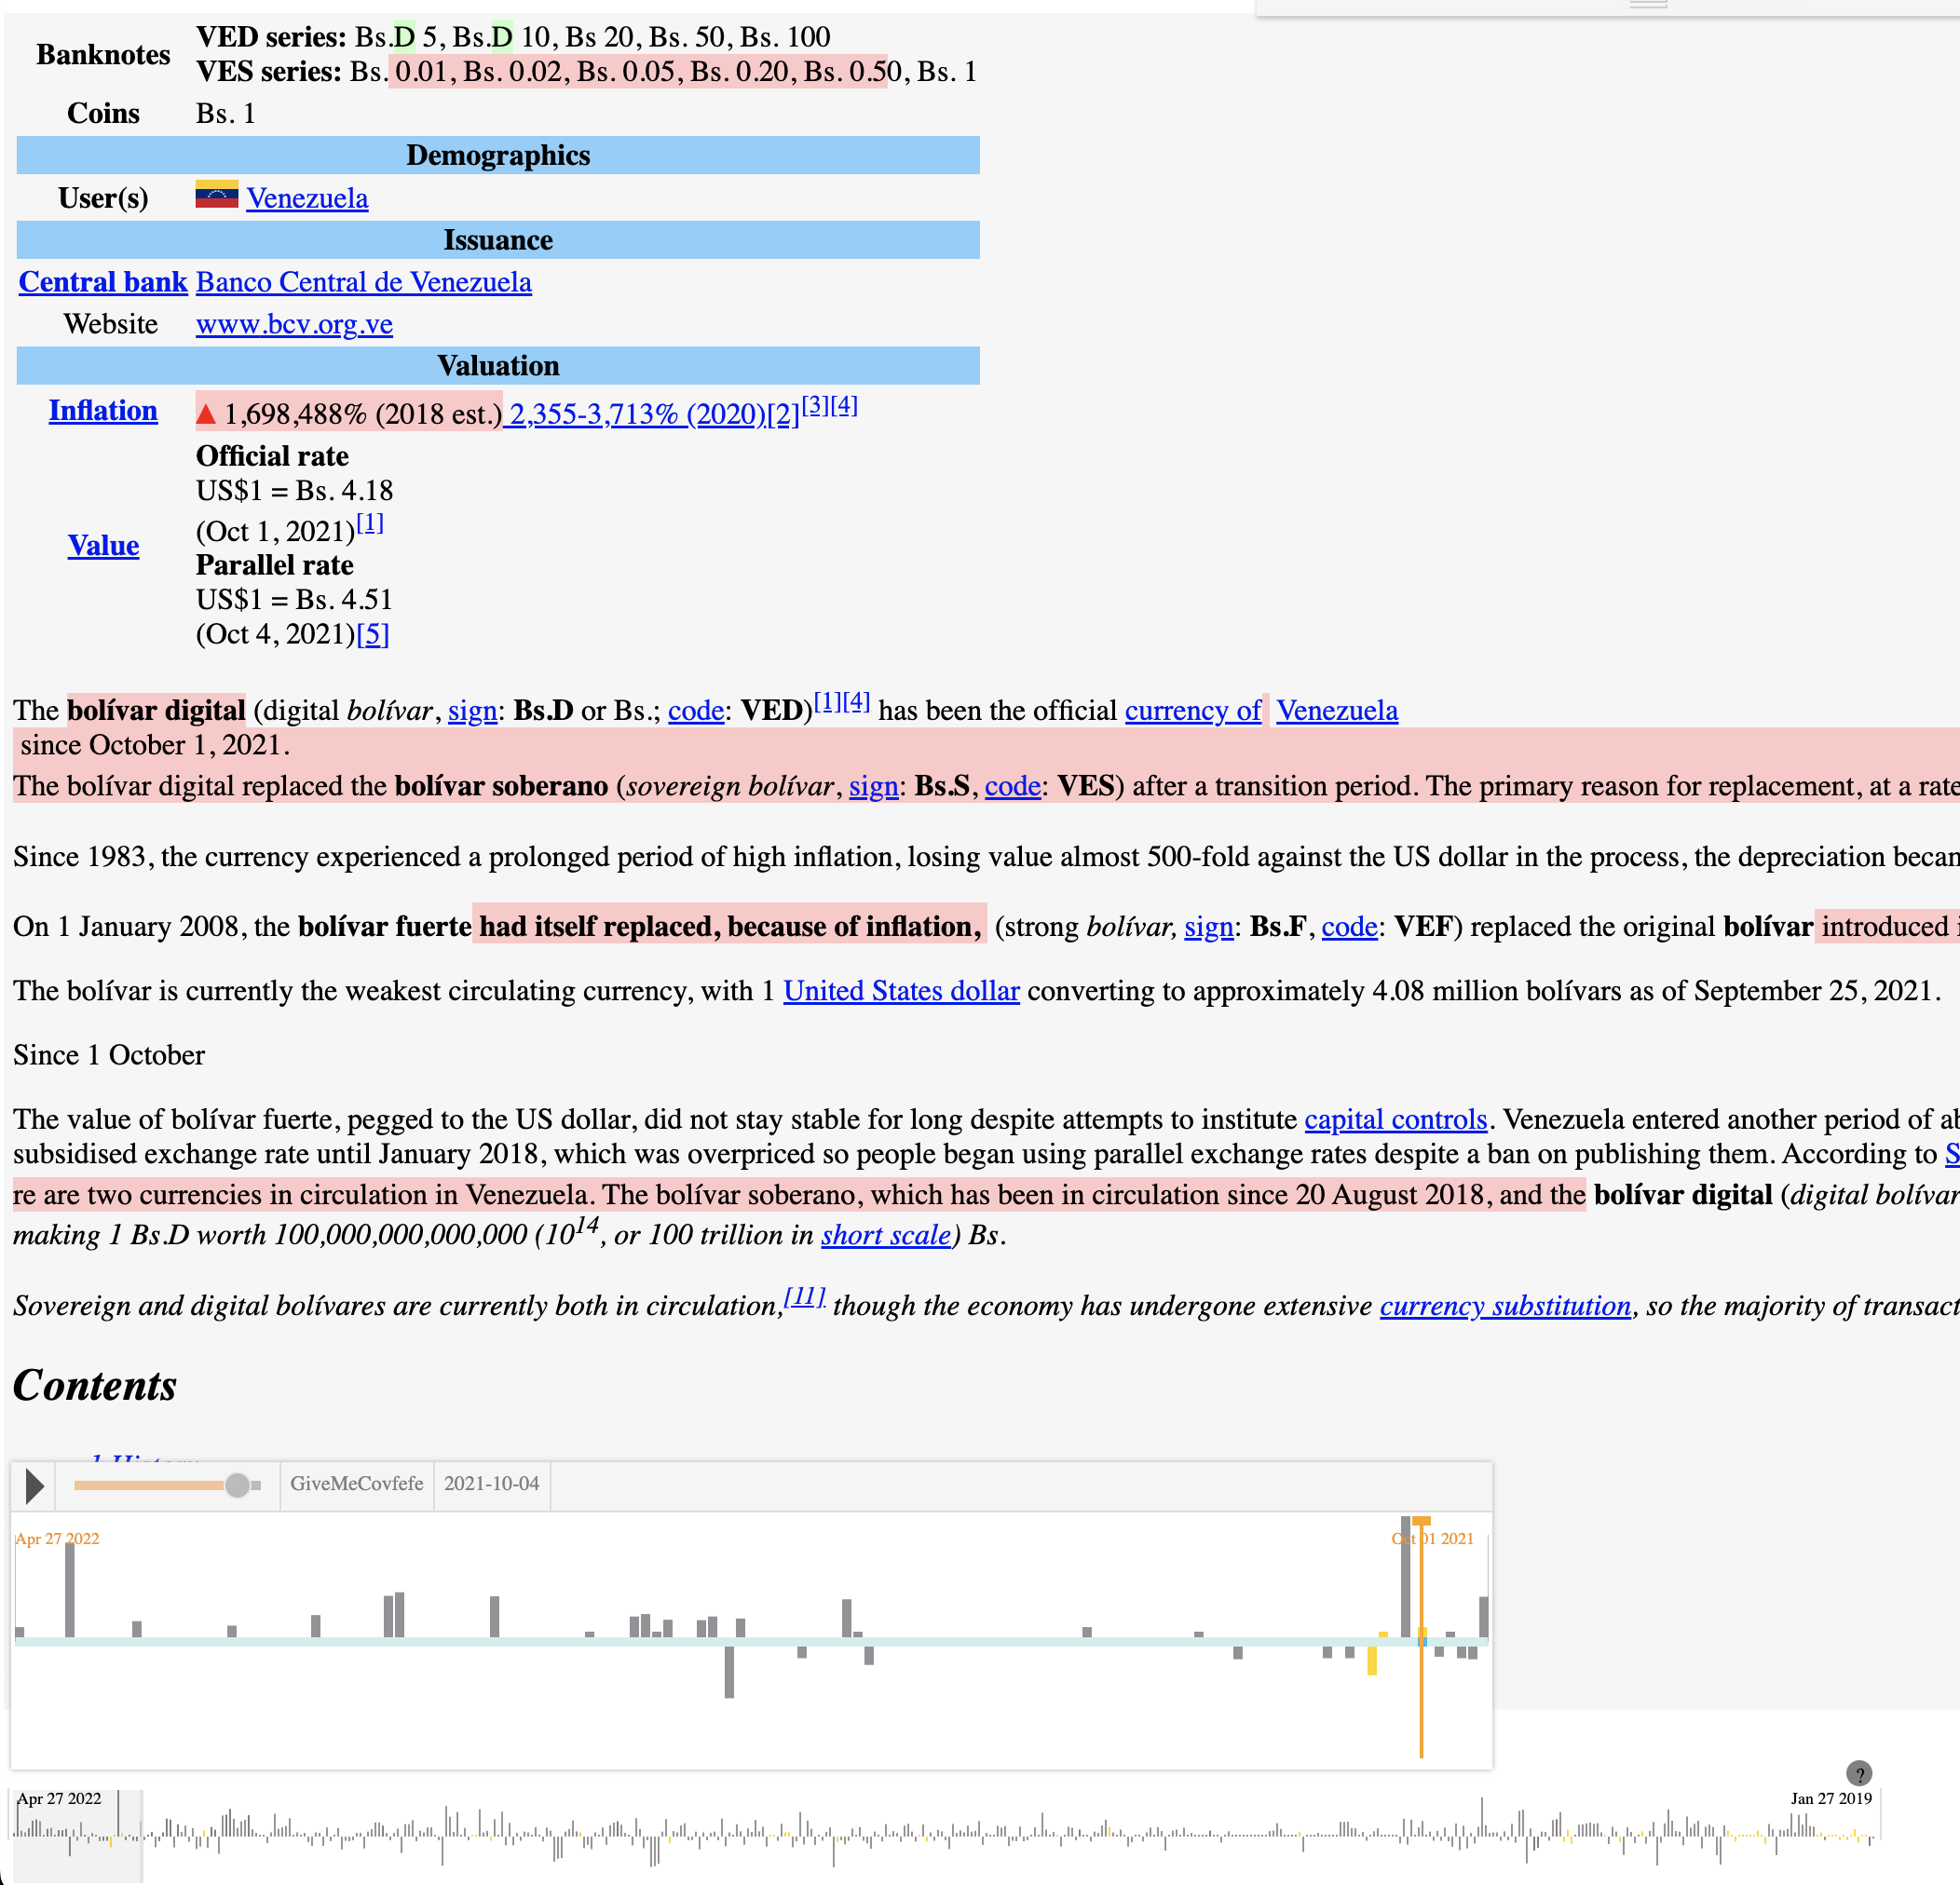
\includegraphics[width=1.0\textwidth]{proyectos relacionados/wikireplay.png}
    \caption{Interfaz de wikireplay}
    \label{wikireplay}
\end{figure}


\url{https://de.wikipedia.org/wiki/Benutzer:Atlasowa/edit_history_visualization}

\subsection{IBM History Flow tool}

\begin{itemize}
    \item URL del proyecto \url{http://alumni.media.mit.edu/~fviegas/papers/history_flow.pdf}
\end{itemize}

Es una herramienta de análisis de datos exploratorio, la cual utiliza el registro de ediciones que posee Wikipedia para mostrar relaciones entre distintas versiones de un documento. El proposito de esta herramienta es mostrar tendencias o patrones generales del documento, pero al mismo tiempo preservar los detalles para una examinación cercana.

Como se puede observar en la imagen \ref*{fig:history-flow-mechanism} cada barra vertical representa una version del documento, siendo el largo proporcional a la cantidad de palabras que posea el documento. El color de cada versión permite asociar cada palabra a un usuario en especifico, identificando a que autor pertenece en dicha versión. Por último se utiliza la distancia entre versiones para separarlas de acuerdo a su fecha y así obtener información extra sobre la frecuencia de edición de cada palabra. Al realizar el procedimiento en la página \say{Brazil} \ref*{fig:brazil-history-flow} se puede observar un evidente incremento en la longitud de las barras verticales, lo que implica un crecimiento drastico del contenido de la pagina.

\begin{figure}[H]
    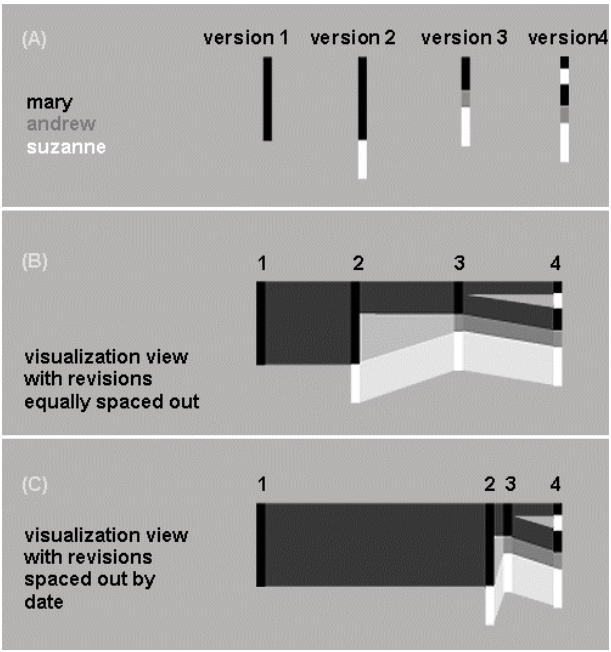
\includegraphics[scale=0.5]{history-flow-mechanism.png}
    \caption{Explicación del mecanismo de visualización de History Flow}
    \label{fig:history-flow-mechanism}
\end{figure}

\begin{figure}[H]
    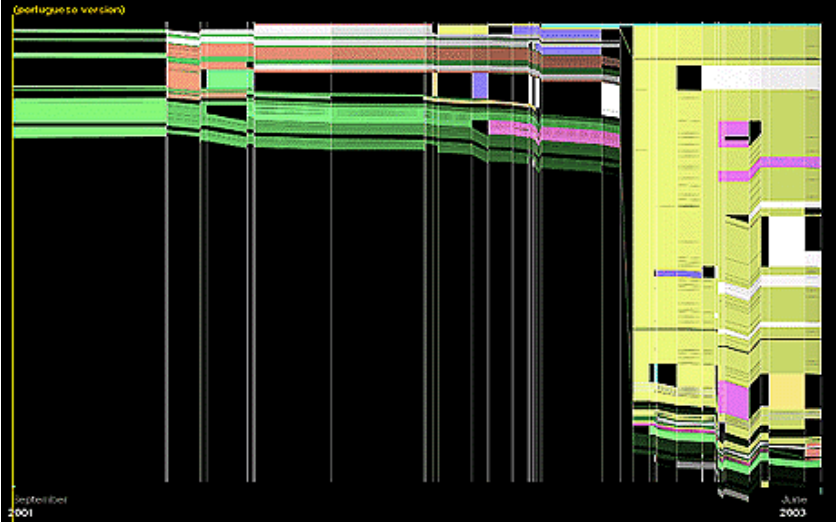
\includegraphics[scale=0.5]{brazil-history-flow.png}
    \caption{La pagina "Brazil" mostrando un crecimiento abrupto y pocas contribuciones anónimas}
    \label{fig:brazil-history-flow}
\end{figure}

\subsection{Wiki History Flow}

\begin{itemize}
    \item URL del proyecto \url{https://github.com/rdmpage/wikihistoryflow}
    \item
\end{itemize}

Este proyecto genera una gráfica de history flow dado el url de un articulo

\section{Herramientas}

\subsection{Tecnologías para el ambiente de desarrollo}
\begin{itemize}
    \item Visual Studio Code.
    \item Git, como control de versiones.
    \item Navegadores web (Google Chrome, Firefox, etc)
    \item Base de Datos (MongoDB)
    \item Servidor (Nodejs)
\end{itemize}

\subsection{Tecnologías o librerías web a utilizar}
\begin{itemize}
    \item Material UI
    \item Next.js + ReactJS
    \item Node
    \item MongoDB
    \item Fastify
\end{itemize}

\section{Requerimientos}
\begin{enumerate}
    \item{Una herramienta capaz de visualizar graficas sobre propiedades de edicion de un wiki.}
    \item{Los wikis a visualizar son extraídas del watchlist del usuario autenticado a traves de Wikipedia (usando API de MediaWiki).}
    \item{Permitir editar las visualizaciones (alternar tipo de grafica, cambiar los tipos de datos a visualizar).}
    \item{Los datos a representar en las visualizaciones son proporcionados a traves del API Wikimetrics 2.0.}
    \item{La herramienta tiene que ser una aplicacion web.}
    \item{La aplicacion tiene que contar con una vista principal que incluya grafica e informacion general de cada uno de los wiki del watchlist.}
    \item{Permitir al usuario crear una visualizacion nueva y guardarla de forma permanente, para este caso es necesario el uso de una base de datos (preferiblemente MongoDB)}
    \item{La aplicación tiene que estar alojada en un servidor, para poder ser accedida de manera remota.}
\end{enumerate}

\section{Prototipo de interfaz}

\subsection{Perfil de Watcher \textbackslash watcher\textbackslash:watcherId}
Para cualquier usuario muestra el perfil de un watcher, en él puedes ver todas las contribuciones de este junto con la lista de visualizaciones que ha creado.
Se permitirá un mínimo de personalización. Y se podrá enlazar el perfil de wikipedia

\begin{figure}[H]
    \centering
    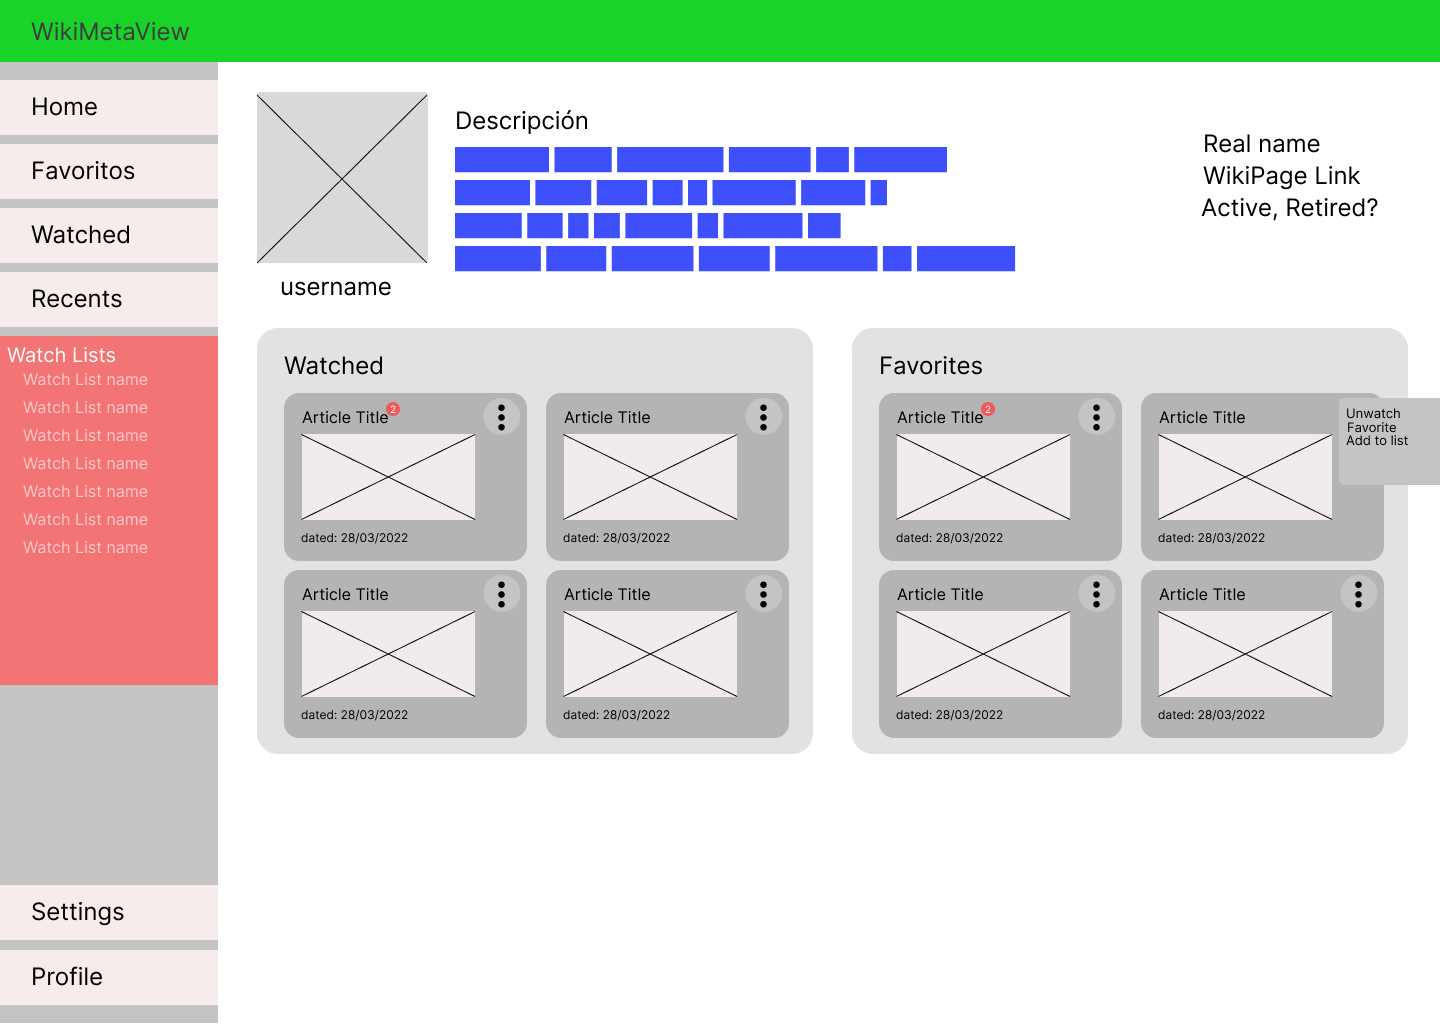
\includegraphics[width=1.0\textwidth]{prototipos/Watcher Profile.png}
    \caption{Prototipo de página de perfil de watcher}
    \label{PrototipoWatchersProfile}
\end{figure}

\subsection{Página principal \textbackslash home}
Para usuarios autenticados, les permite ver diferentes secciones relevantes para ellos

\begin{figure}[H]
    \centering
    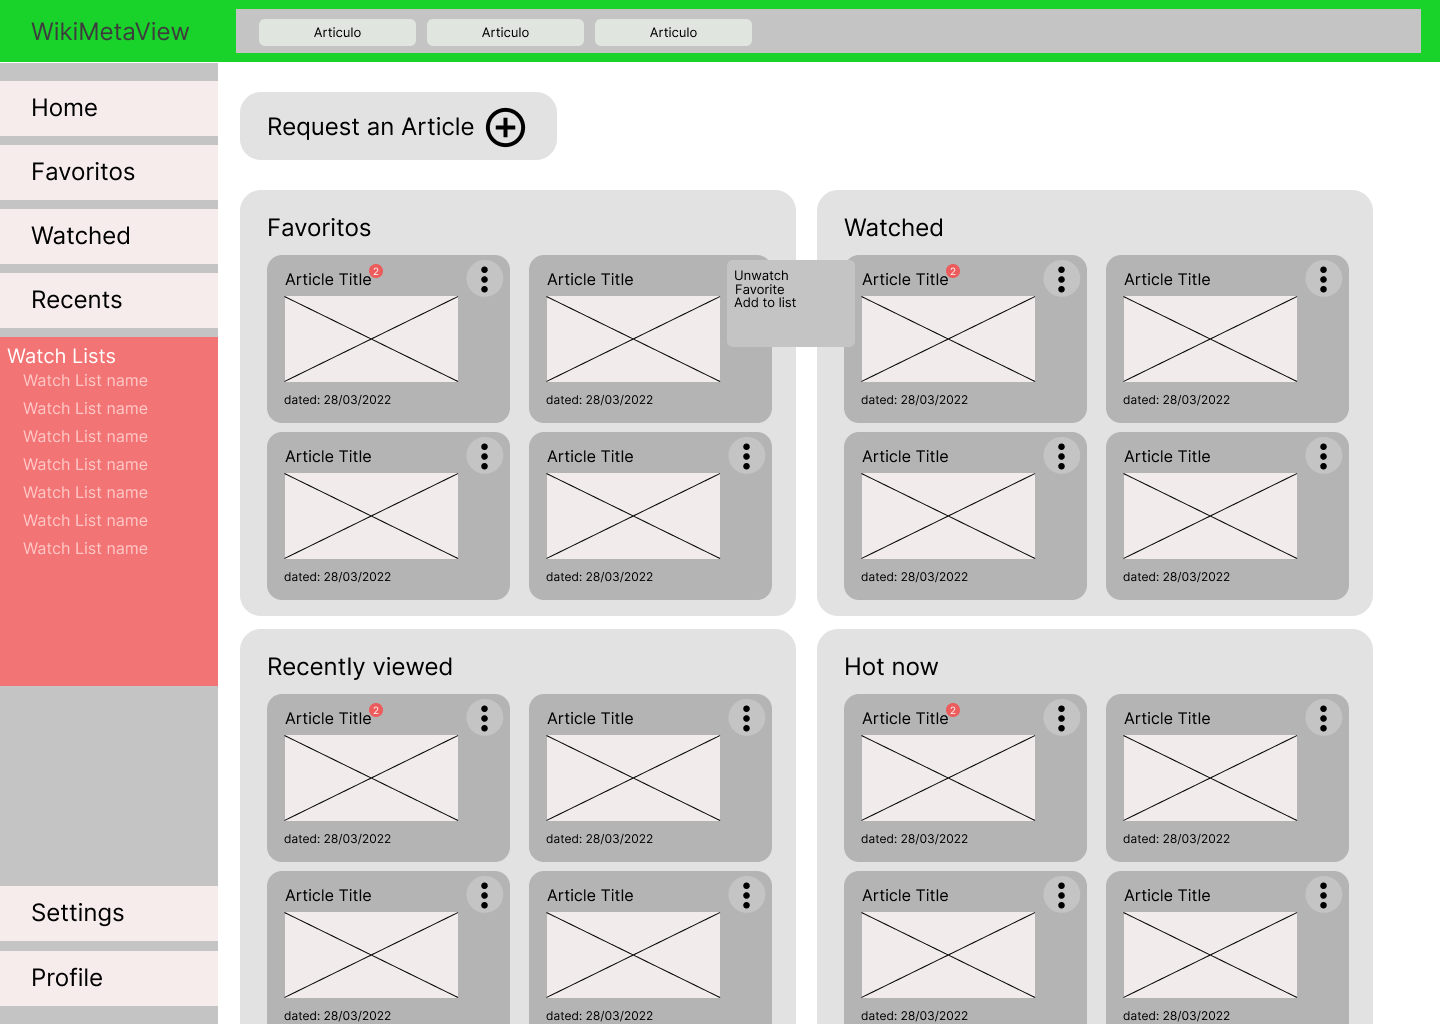
\includegraphics[width=1.0\textwidth]{prototipos/Index Auth.png}
    \caption{Prototipo de vista principal de un usuario autenticado}
    \label{PrototipoHomePage}
\end{figure}


Secciones del home
\begin{enumerate}
    \item Watched \\ Muestra una lista y un pequeño abstracto de los artículos que el usuario hace watching y tienen una visualización actualizada
    \item Queue \\ Muestra una lista de los artículos que le usuario solicito para hacer una visualización pero que el server no ha podido solicitar
    \item Controversial \\ Muestra una lista de aquellas visualizaciones que provocan discusión en la comunidad, caracterizado por muchos comentarios
\end{enumerate}

\subsection{Landing page \textbackslash}
TODO: poner imagen
Esta pagina se encarga de explicar las motivaciones de la App y dar una noción básica del funcionamiento para los watchers.
Tiene el objetivo de cap

\subsection{Página de configuración \textbackslash settings}
TODO: Terminar seccion de settings
Acá el usuario puede bla bla

\subsection{Página de artículo \textbackslash article}
\url{/article?title=<title>&url=<url>}
Muestra un articulo junto con su metadata y las visualizaciones creadas por los usuarios.d

\begin{figure}[H]
    \centering
    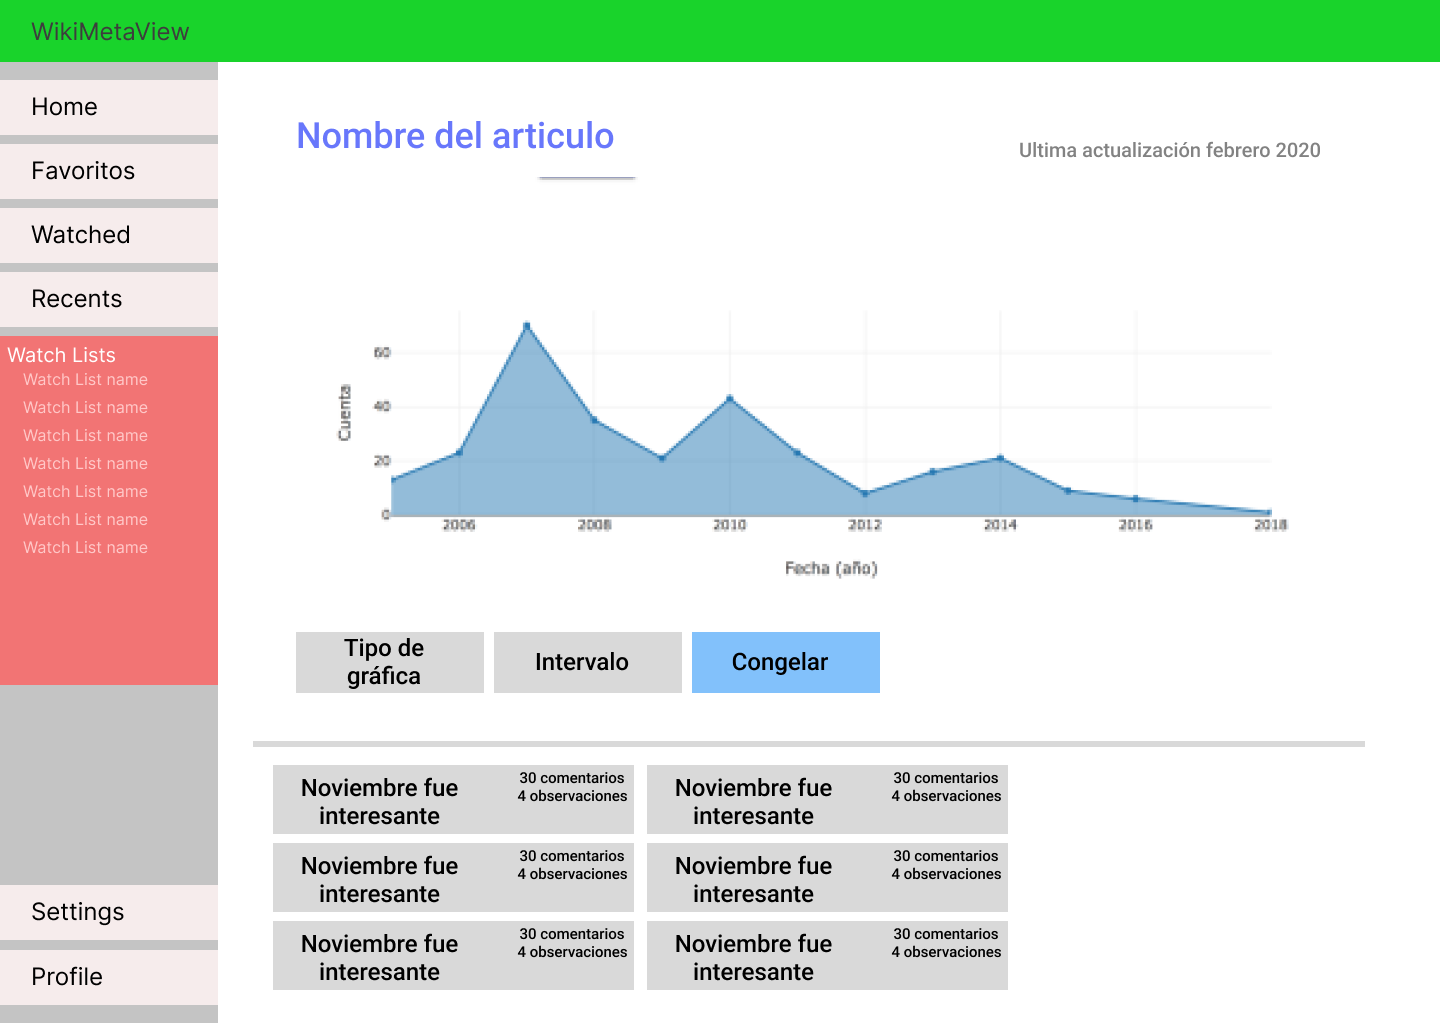
\includegraphics[width=1.0\textwidth]{prototipos/Article Page.png}
    \caption{Prototipo de página de artículos}
    \label{PrototipoSettingsPage}
\end{figure}

\subsection{Sobre nosotros \textbackslash about}
Breve resumen del proyecto, incluye el documento de tesis y documento de seminario asi como datos de contacto y repositorios de github para futuros contribuyentes.

\section{Modales}
Las modales pueden sobreponerse a cualquier página en la aplicación y permiten al usuario efectuar una acción.

Estas modales serán controladas por parámetros de consulta agregados al URL de cada página web
CleanArquitecture
\subsection{Modal de autenticación}

Si este parámetro esta en el url. Presenta la modal de autenticación

\begin{figure}[H]
    \centering
    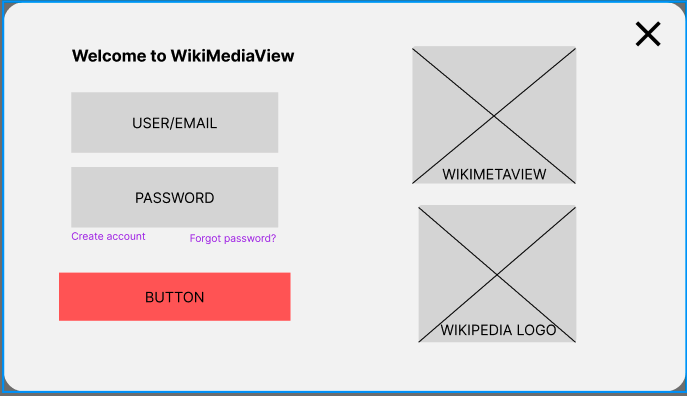
\includegraphics[width=1.0\textwidth]{prototipos/Modal-Auth.png}
    \caption{Modal de autenticación}
    \label{ModalAuth}
\end{figure}
?auth=true

\section{Planificación de las actividades}

TODO: UNA TABLA DE DOS COLUMNAS

ACTIVIDAD, TIEMPO ESTIMADO.

\begin{lstlisting}
    Preparar el entorno de desarrollo 1/2 semana
    Estudiar API Wikimetrics 2.0 (Back-end) 1/2 semana
    Estudiar API MediaWiki 1/2 semana
    Integracion del API Wikimetrics 2.0 (Back-end) 1/2 semana
    Integracion del API MediaWiki 1/2 semana
\end{lstlisting}

\printbibliography

\end{document}